\subsection{Mesh Topology}
SHOCK uses a powerful mesh topology containing subzones with rotated coordinate systems.
By using the example of an triangle, this features is explained.
\par
Figure~\ref{fig:triangle} sketches the considered geometry of the isosceles triangle.

\begin{figure}[!ht]
  \begin{center} 
    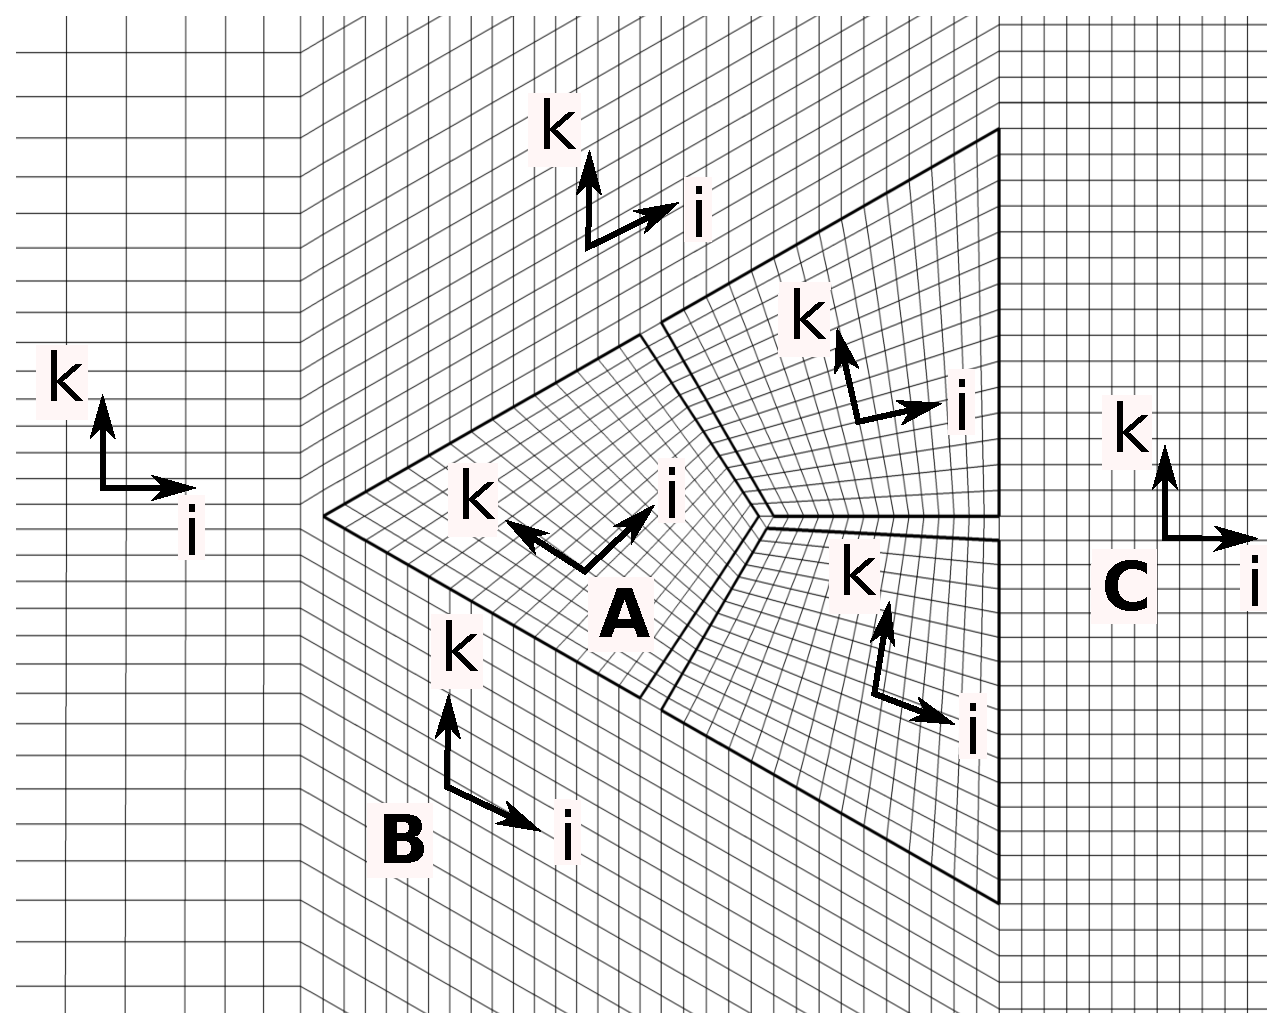
\includegraphics[width=0.7\linewidth]{grid_transformation}
  \end{center}
  \caption {mesh cut through triangle}
  \label{fig:triangle}
\end{figure}

By adapting the mesh to the triangle, the number of mesh points for these edges are interdependent.
That is why the number of mesh points for all three sides is constant.
While using a structured mesh, the generation of a mesh which takes the triangle into account is a challenging task.
Immersed boundaries are an easy solution if complex geometries have to be considered in structured meshs.
The disadvantage of the immersed boundaries in conjunction with triangles is that the mesh line crossing oblique edges cannot be represented smoothly.
Depending on the local mesh resolution the resulting boundaries are more or less serrated.
This effect is called sawtooth distortion or aliasing.
In order to avoid this disadvantage another solution is presented.
The triangle is exactly modelled if it is replaced by three quadrilateral.
Now, the mesh lines represent exactly the edges of the triangle improving the smoothness of the solution.
Connecting the different parts of the mesh around the triangle, in Fig.~\ref{fig:triangle} it is apparent, that only \textit{non-easy} mesh topologies are possible.
Some adjacent zones, i.e. zone A and B in Fig.~\ref{fig:triangle}, use differently oriented coordinate systems.
Consequently, to allow rotated coordinate systems, the introduction of a transformation matrix between the zones is necessary.
It has to be noted, that besides the advantages of a more generalized mesh topology containing transformation matrices, the Message Passing Interface (MPI)-communication becomes more complex.
While a simple rectangular mesh allows the use of a \textit{Cartesian Communicator} and a synchronous MPI-communication (MPI-Sendrecv), the mesh shown in Figure~\ref{fig:triangle} is not compatible, because the identification of the neighbors is no longer unique.
Looking in the i-direction, the zone B is the lower neighbor of the zones A and C.
As a consequence, the communication is changed into an asynchronous one (MPI-Isend/MPI-Irecv).
Further, instead of a global, \textit{Cartesian Communicator}, now the mesh, or rather the interfaces provide the information about communication partners that are connected via the interfaces.

\subsection{Memory}
In the following, the memory management is considered.
First of all, it is important to note, that SHOCK has no master process.
Every thread uses nearly the same amount of memory.
Considering one mesh point, nearly 300 double precision variables are allocated.
This also includes variables for saving transient data.
The memory cost besides these variables is negligible.

\subsection{I/O}
The I/O of SHOCK is limited to the start and the end of the simulation.
A file format for CFD data (CGNS [CFD General Notation System], using HDF5, \cite{Pakalapati2005} ) supports the comfortable handling of big amount of data.
In a bachelor thesis \cite{Sodhi2013}, the parallel CGNS commands were implemented which enables SHOCK to use one single cgns-file containing the data for all threads instead one file for each thread.
This dramatically simplifies the data management since a data post processing is not needed any more.
SHOCK's results can be transferred continuously from the production system.


\subsection{Parallelization \& scalabilty}
SHOCK is parallelized with pure MPI (Message Passing Interface), in order to carry out simulations with large numerical costs in a realistic time.
A hybrid parallelization was tested but showed no benefit and therefore, it was deactivated.
The communication is asynchronous since the mesh topology enables rotated coordinate systems.
In such cases, a synchronous communication (i.e. all send to left and receive from right) is not possible.
Nevertheless, the general mesh topology has great advantages since it is not limited to simple meshes and the scalability of the code is not significantly worse which is shown in the following.
\par
On JUQUEEN using 32 threads per node (pure MPI code), scalability tests have been performed in order to demonstrate that the code is appropriate to be used for a massive parallelization.
On a three dimensional grid consisting of $16\cdot 10^6$ grid points (256x256x256) a test simulation with 500 time steps was conducted.
Figure~\ref{scale} illustrates the results for five levels of parallelization.
Starting with 512 cores while the number of cores was doubled from one level to the next.
The highest number of cores that was considered in this scaling test is 8,192.
In general, the code can run on further levels of parallelization (recent record (23.11.2014): 262,144 threads), but for the used grid a further decomposition was not meaningful.
The relation of the number of ghost points, which define the communicated data, and the number of grid points, where the solution is computed, rises up to a value of 4.06 for the highest level of decomposition.
As a result the communication time takes 17.8 \% of the absolute time for this level.
Assuming a cubic decomposition, the number of ghost points $GHP$ and grid points $GRP$ per thread are approximated by $GRP=256^3/no.\ threads$ and $GHP=(GRP^{1/3}+2\cdot N)^3-GRP$ with $N=3$ for the used spatial order.

\begin{table}[H]
\centering
\begin{tabular}{c|c|c|c|c}
\textbf{cores} & \textbf{time (s)} & \textbf{comm. time (s)} & $GHP/GRP$ & \textbf{speedup}\\ 
\hline 
512 & 1,166 & 46 [3.9\%]& 1.89 & 1.0\\
1,024 & 598 & 36 [6.1\%]& 2.18 & 1.9\\
2,048 & 316 & 27 [8.6\%]& 2.6 & 3.7\\
4,096 & 171 & 23 [13.5\%]& 3.2 & 6.8\\
8,192 & 94 & 17 [17.8\%]& 4.06 & 12.4\\ 
\end{tabular} 
\end{table}

\begin{figure}[H]
\centering
{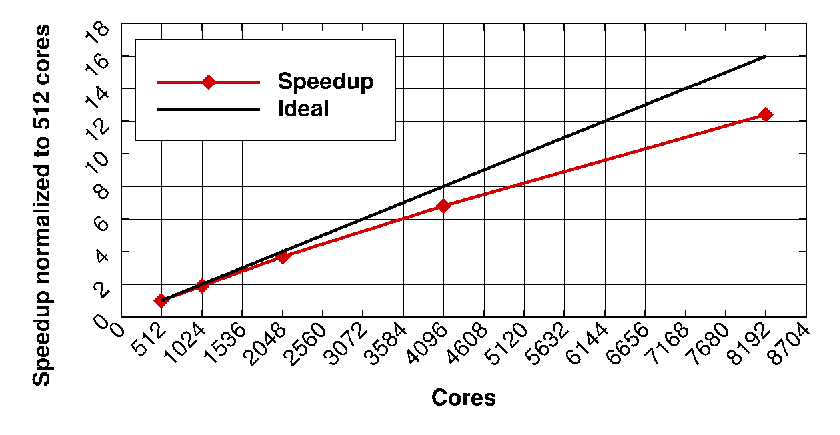
\includegraphics[width = 0.7\linewidth]{scale.eps}}
\caption{Scaling behaviour of SHOCK (WENO $5^{th}$ and Runge-Kutta $3^{rd}$ order) on JUQUEEN (256x256x256 grid points and 500 time steps). Speedup is normalized to 512 cores.}
\label{scale}
\end{figure}
